\documentclass[a4paper]{resume}

\ResumeName{LAI JING}
\usepackage{graphicx}
\usepackage{tikz}
\usepackage{enumitem}

% 极致紧凑排版优化
\setlist[itemize]{leftmargin=1.2em, itemsep=0pt, parsep=0.1em, topsep=0pt}
\makeatletter
\let\cleardoublepage\clearpage
\makeatother

\begin{document}

\ResumeContacts{
  (+86) 188-1158-9056,%
  \ResumeUrl{mailto:3058243931@qq.com}{3058243931@qq.com}
}

\begin{tikzpicture}[remember picture, overlay]
  \node [anchor=north east, inner sep=0.8cm] at (current page.north east) 
    {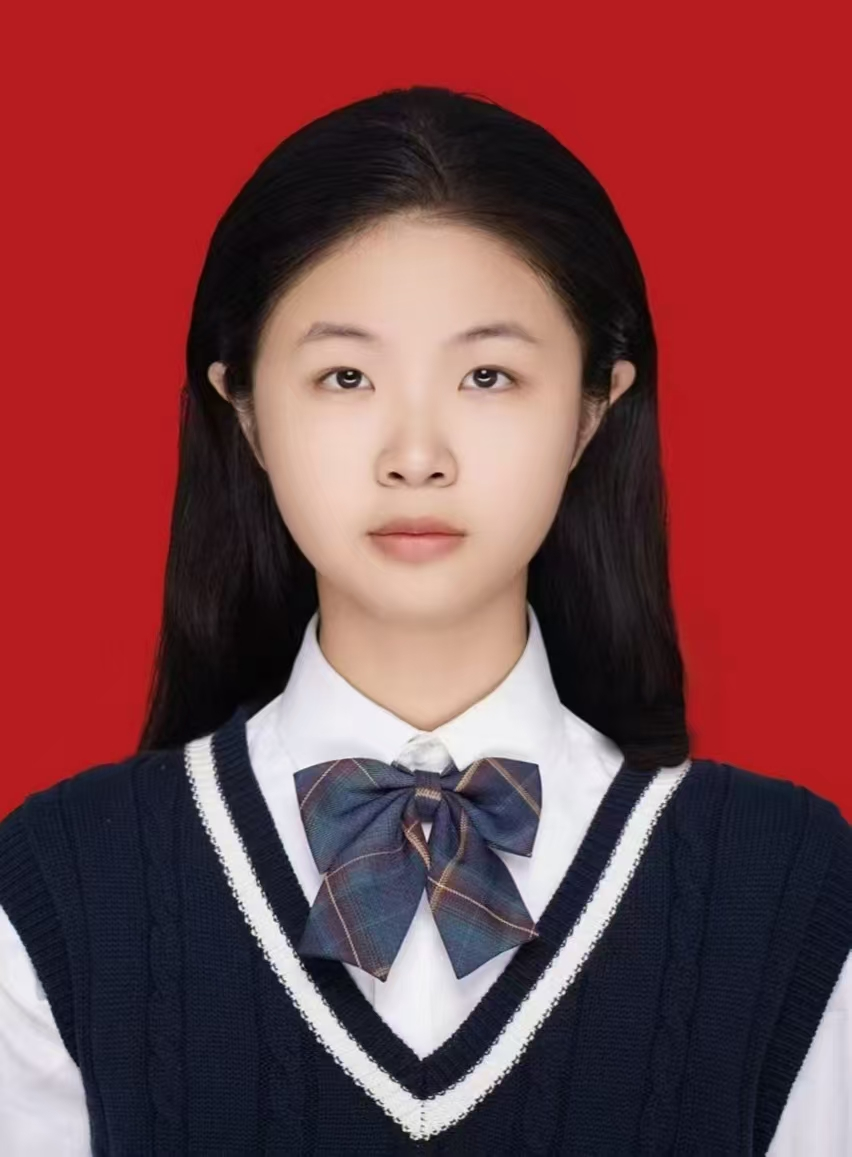
\includegraphics[width=1.8cm]{head.jpg}};
\end{tikzpicture}

\ResumeTitle

\section{Education}
\ResumeItem[Education]{University of International Business and Economics (UIBE)}[Dual B.A. in Int'l Politics \& English][Sept. 2024 -- June 2028]
\begin{itemize}
    \item \textbf{Academic Performance}: Ranked \textbf{1/89} in the School of International Relations; GPA \textbf{3.94/4.00}; Average Score \textbf{91.33}.
    \item \textbf{Honors}: National Encouragement Scholarship; Bronze Prize of "Understanding Contemporary China" (Provincial Level).
\end{itemize}

\section{Internship Experience}

\ResumeItem[CCG]{Center for China and Globalization (CCG)}[Global Young Leaders Dialogue (GYLD) Intern][Jan. 2026 -- Present]
\begin{itemize}
    \item \textbf{Conference Coordination}: Involved in "GYLD Annual Dialogue" and "Global Distinguished Speakers Dialogue" with UNICEF; managed cross-departmental communication and drafted high-level bilingual meeting minutes.
    \item \textbf{Media Matrix Operation}: Managed official WeChat and YouTube channels for GYLD and Global Talent Organization Federation; conducted daily content production and multi-platform data analysis.
    \item \textbf{Foreign Affairs Translation}: Provided language support for high-profile events, including translating English speeches for foreign guests in Tongzhou and official documents for delegations to Switzerland and Austria.
\end{itemize}

\ResumeItem[MOFCOM]{Ministry of Commerce of the P.R.C. (MOFCOM)}[Foreign Aid Training Assistant][Nov. 2025 -- Dec. 2025]
\begin{itemize}
    \item \textbf{Bilingual Documentation}: Responsible for translating and proofreading training manuals for the "Workshop on Global Climate Governance," ensuring the accuracy of diplomatic terminology and formal formatting.
    \item \textbf{Coordination}: Assisted officials in managing foreign participants and executing cultural exchange activities; established \textbf{training data archives} to optimize project efficiency.
\end{itemize}

\ResumeItem[PSR]{Political Science Review}[External Communication Intern][Sept. 2025 -- Present]
\begin{itemize}
    \item \textbf{Content Curation}: Tracked international political hotspots and assisted in topic selection; screened and translated core academic literature from foreign journals into accessible Chinese articles.
    \item \textbf{Editorial Management}: Managed final layout and typography for social media推文; strictly controlled image quality and formatting details to ensure professional presentation.
\end{itemize}

\ResumeItem[NSCL]{National Security Computing Lab, UIBE}[Research Assistant][July 2025 -- Dec. 2025]
\begin{itemize}
    \item \textbf{Industrial Research}: Researched BRICS new energy industrial cluster cooperation mechanisms, systematically organizing data for \textbf{six countries} including Russia, Brazil, and Saudi Arabia.
    \item \textbf{Reporting}: Conducted comparative analysis on cluster characteristics and drafted reports on \textbf{Sino-foreign industrial cooperation paths}, which were officially recognized by the \textbf{MIIT}.
\end{itemize}

\section{Campus Activities}

\ResumeItem[Challenge Cup]{"Echoes of the Journey" Cultural Project}[Project Leader (Challenge Cup)][Nov. 2024 -- April 2025]
\begin{itemize}
    \item Proposed "Immersive Script-kill + Red Education" concept; built multi-thread narrative models and drafted business plans.
\end{itemize}

\ResumeItem[Youth League]{University Youth League Committee}[Project Department Staff][Sept. 2025 -- Present]
\begin{itemize}
    \item Managed "Challenge Cup" applications; established Excel-based monitoring systems for cross-school collaboration and compliance.
\end{itemize}

\section{Core Skills}
\begin{itemize}
  \item \textbf{Languages}: English (Working Proficiency, C1), Mandarin (Native), French (Basic).
  \item \textbf{Technical}: Proficient in R (Data Cleaning \& Modeling), AI Prompt Engineering, and Adobe Premiere Pro.
  \item \textbf{Design}: Skilled in WeChat layout tools (Xiumi/Canvas) and video editing (Jianying/Premiere).
\end{itemize}

\end{document}
